%! Author = Len Washington III
%! Date = $\frac{3}{20}$/2024

% Preamble
\documentclass[title={Chapter 11}]{fdsn201notes}

% Packages

% Document
\begin{document}%
%
%<*Chapter11>
\maketitle{11}{}%

\section{Physical Activity and Fitness}\label{sec:physical-activity-and-fitness}
\begin{itemize}
	\item \definition{Physical activity}{any muscle movement that increases energy expenditure}
	\item \definition{Leisure-time physical activity}{any activity unrelated to a person’s occupation}
	\begin{itemize}
		\item For example, hiking, walking, biking
		\item Includes \definition{exercise}{purposeful, planned physical activity}
	\end{itemize}
	\item The components of physical fitness are achieved through three types of exercise
	\begin{itemize}
		\item Aerobic exercise
		\item Resistance training
		\item Stretching
	\end{itemize}
	\item \definition{Physical fitness}{the ability to carry out daily tasks with vigor and alertness, without undue fatigue, and with ample energy to enjoy leisure-time pursuits and meet unforeseen emergencies}
	\begin{itemize}
		\item The components of physical fitness are
		\begin{itemize}
			\item Cardiorespiratory fitness
			\item Musculoskeletal fitness
			\item Flexibility
			\item Body composition
		\end{itemize}
	\end{itemize}
\end{itemize}

\begin{table}[H]
	\centering
	\begin{threeparttable}
		\caption{Components of Fitness}
		\label{tab:components-of-fitness}
		\rowcolors{2}{rowmedgreen}{rowlightgreen}
		\begin{tabular}{p{0.26\textwidth} p{0.74\textwidth}}
			\rowcolor{rowdarkgreen}\textbf{Fitness Component} & \textbf{Recommended Intake}\\
			Cardiorespiratory & Examples of Activities that Improve Fitness in Each Component Aerobic-type activities, such as walking, running, swimming, cross- country skiing\\
			Musculoskeletal fitness: & Resistance training, weight lifting, calisthenics, sit-ups, push-ups\\
			\rowcolor{rowmedgreen}Muscular strength & Weight lifting or related activities using heavier weights with few repetitions\\
			\rowcolor{rowmedgreen}Muscular endurance & Weight lifting or related activities using lighter weights with more repetitions\\
			Flexibility & Stretching exercises, yoga\\
			Body composition & Aerobic exercise, resistance training\\
			\rowcolor{rowdarkgreen} & \\
		\end{tabular}
		\begin{tablenotes}
			\small
			\item
		\end{tablenotes}
	\end{threeparttable}
\end{table}

\section{Physical Activity and Chronic Disease}\label{sec:physical-activity-and-chronic-disease}
\begin{itemize}
	\item Regular physical activity
	\begin{itemize}
		\item Reduces the risk of heart disease, stroke, and high blood pressure
		\item Reduces the risk of obesity
		\item Reduces the risk of type 2 diabetes
		\item May reduce the risk of colon cancer
		\item Reduces the risk of osteoporosis
	\end{itemize}
\end{itemize}

\begin{figure}[H]
	\centering
	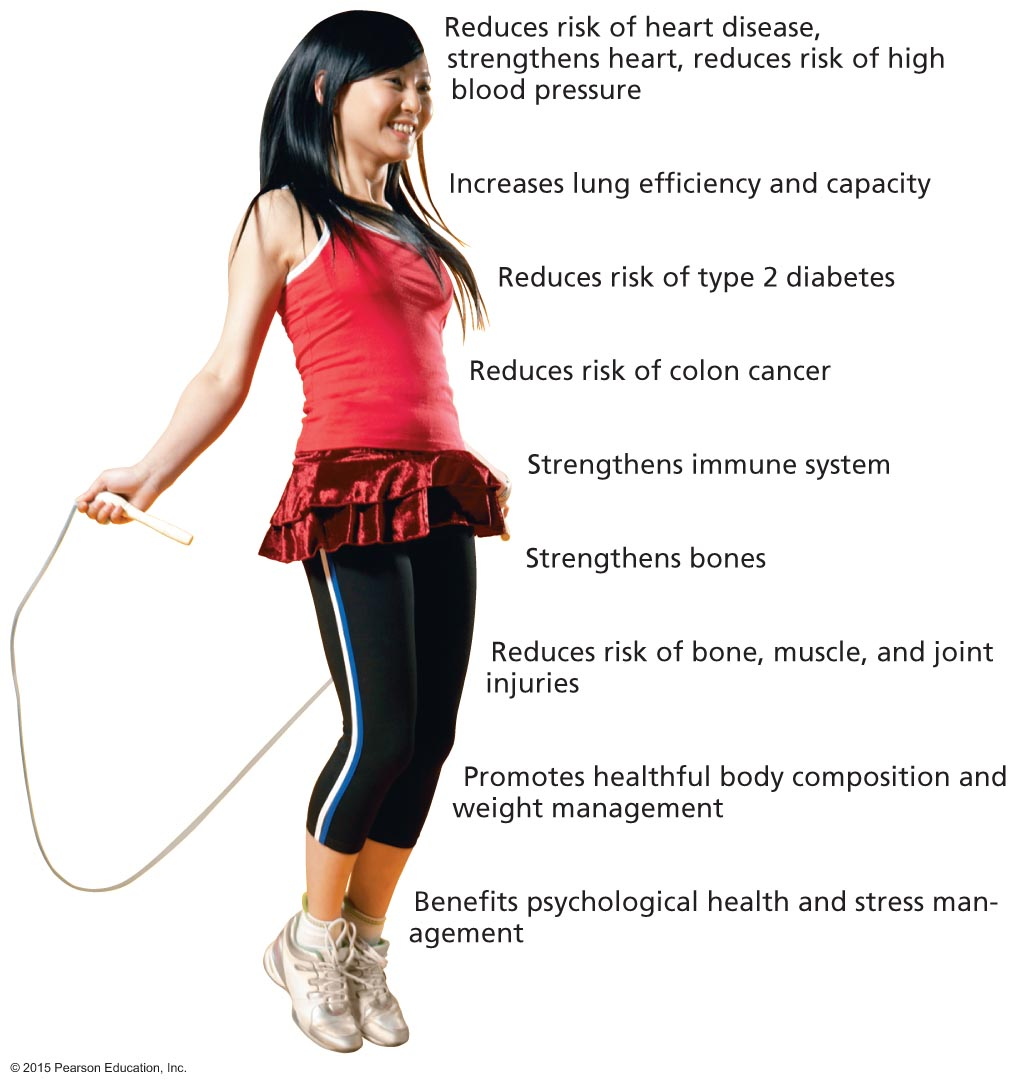
\includegraphics[width=\textwidth]{11_health_benefits_of_physical_activity}
	\caption{Health Benefits of Physical Activity}
	\label{fig:health-benefits-of-physical-activity}
\end{figure}

\section{Physical Activity and Most Americans}\label{sec:physical-activity-and-most-americans}
\begin{itemize}
	\item Despite the clear benefits of regular physical activity,
	\begin{itemize}
		\item 79.9\% of U.S.\ adults do not perform sufficient physical activity
		\item 23.7\% of U.S.\ adults admit to doing no leisure-time physical activity at all
	\end{itemize}
\end{itemize}

\nutrients{Rates of Physical Activity in the United States}{tab:rates-of-physical-activity-in-the-united-states}

\section{Designing a Sound Fitness Program}\label{sec:designing-a-sound-fitness-program}
\begin{itemize}
	\item For a sound fitness program:
	\begin{itemize}
		\item Start by assessing your current level of fitness
		\item Identify your personal fitness goals
		\item Make your program varied, consistent, and fun
		\item Appropriately overload your body
		\item Include a warm-up and cool-down period
		\item Start out slowly and gradually build up the time you spend each day until you reach 30 minutes
	\end{itemize}
\end{itemize}

\section{Sound Fitness Program}\label{sec:sound-fitness-program}
\begin{itemize}
	\item A sound physical fitness program meets your personal fitness goals
	\item An individual’s fitness program may vary depending on whether he or she is
	\begin{itemize}
		\item Training for athletic competition
		\item Working toward cardiorespiratory fitness
		\item Trying to maintain overall health
	\end{itemize}
	\item A sound physical fitness program is fun
	\item An individual’s fitness program should focus on what he or she enjoys
	\begin{itemize}
		\item Outdoor activities
		\item Social recreation
	\end{itemize}
	\item A sound physical fitness program includes variety and consistency
	\item Variety can be achieved by
	\begin{itemize}
		\item Combining aerobic exercise, resistance training, and stretching
		\item Combining indoor and outdoor exercises
		\item Taking different routes when walking or jogging
		\item Including entertainment such as music
		\item Participating in different activities each week
	\end{itemize}
	\item A sound physical fitness program appropriately overloads the body
\end{itemize}

\definition{Overload principle}{put additional physical demands on the body to improve fitness}
\begin{itemize}
	\item Too much physical exertion is not recommended
	\item The \emph{FITT principle} can be used to determine appropriate overload
\end{itemize}

\section{The FITT Principle}\label{sec:the-fitt-principle}
\begin{description}
	\item[Frequency:] the number of activity sessions per week
	\begin{itemize}
		\item Desired frequency varies with fitness goals
	\end{itemize}
	\item[Intensity:] the amount of effort expended or how difficult the activity is to perform
	\begin{itemize}
		\item Desired intensity may be based on maximal heart rate
	\end{itemize}
	\item[Time of activity:] how long each session lasts
	\item[Type of activity:] the range of activities engaged in to promote health and physical fitness
\end{description}

\begin{figure}[H]
	\centering
	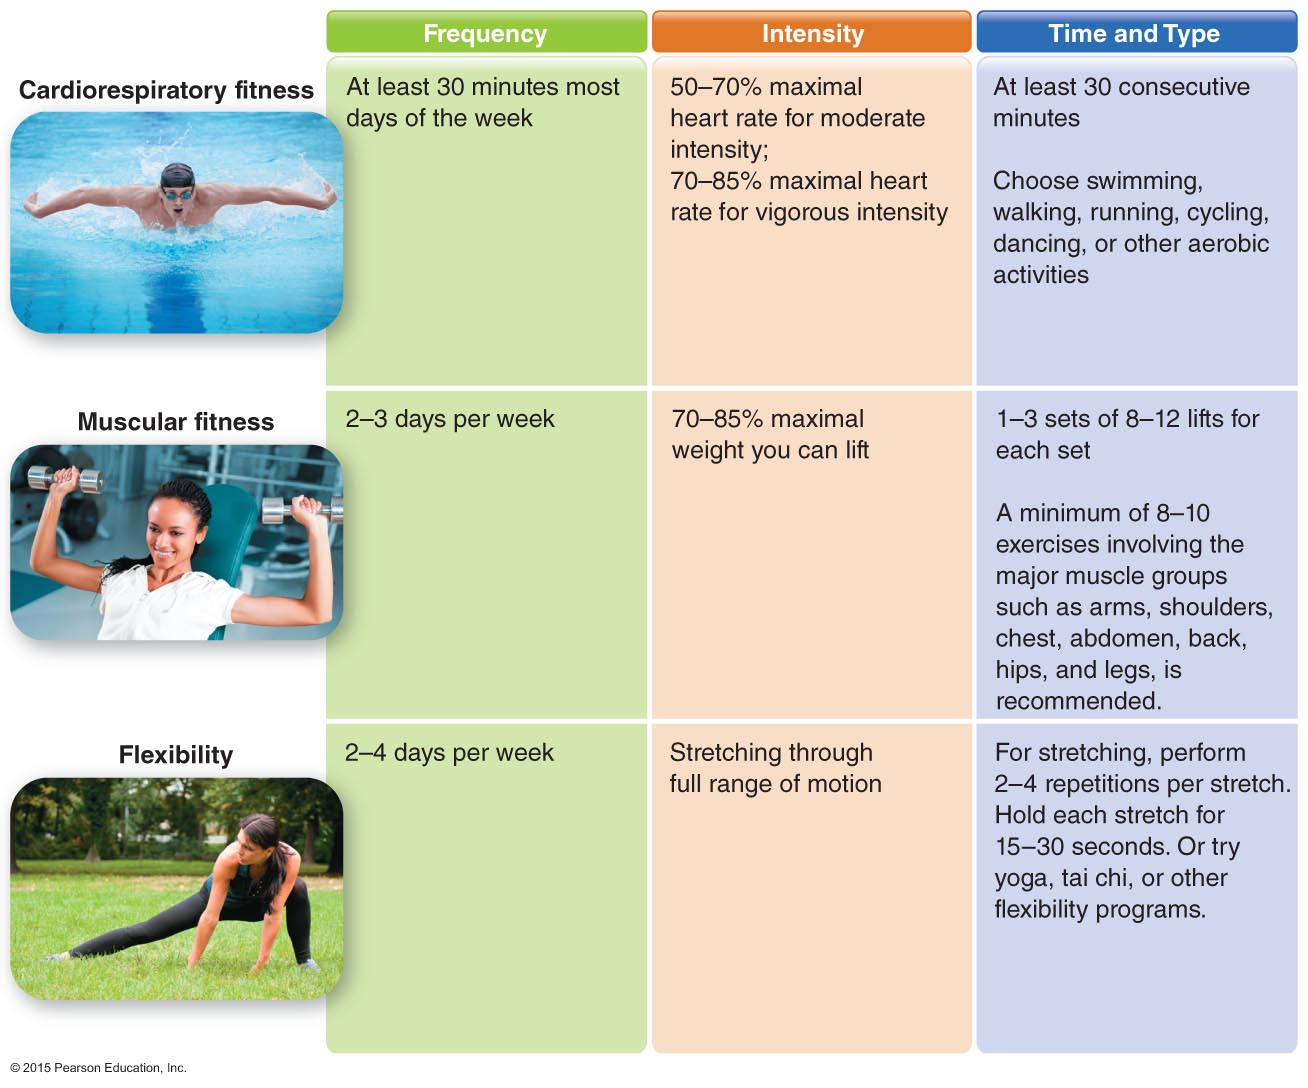
\includegraphics[width=\textwidth]{11_using_the_fitt_principle}
	\caption{Using the FITT Principle}
	\label{fig:using-the-fitt-principle}
\end{figure}

\begin{figure}[H]
	\centering
	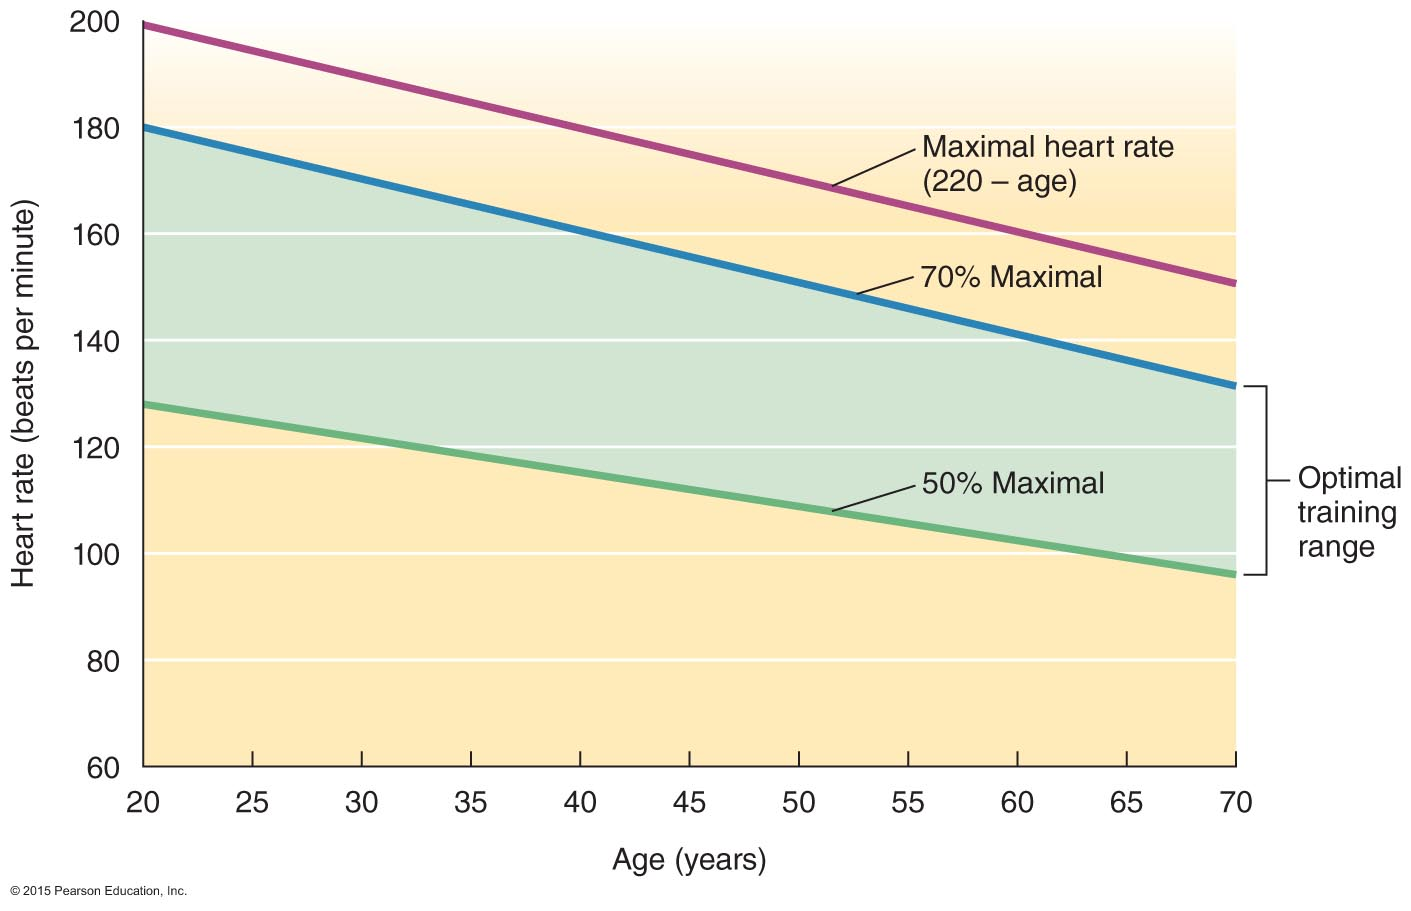
\includegraphics[width=\textwidth]{11_maximal_heart_rate_training_chart}
	\caption{Maximal Heart Rate Training Chart}
	\label{fig:maximal-heart-rate-training-chart}
\end{figure}

\section{Sound Fitness Program}\label{sec:sound-fitness-program-2}
A sound physical fitness program includes a warm-up period and a cool-down period

\subsection{Warm-Up}\label{subsec:warm-up}
\begin{itemize}
	\item Should be brief (5 to 10 minutes), gradual, and sufficient to increase muscle and body temperature
	\item Includes aerobics, calisthenics, and stretching
	\item Enhances flexibility and helps prepare you psychologically for the activity to come
\end{itemize}

\subsection{Cool-down}\label{subsec:cool-down}
\begin{itemize}
	\item Should be gradual
	\item Includes some of the same activities as in the exercise session, along with stretching
	\item Assists in preventing injury and may help reduce muscle soreness
\end{itemize}

\section{Fuel for Physical Activity}\label{sec:fuel-for-physical-activity}
\begin{itemize}
	\item The common currency for energy in the body is \emph{adenosine triphosphate}, or \emph{ATP}
	\item After depleting ATP stores, muscles turn to other energy sources
	\begin{itemize}
		\item \emph{Creatine phosphate (CP)} stores energy that can be used to generate ATP
		\begin{itemize}
			\item Creatine phosphate can be broken down to support the regeneration of ATP for enough energy for 3--15 seconds of maximal physical effort
		\end{itemize}
	\end{itemize}
\end{itemize}

\begin{figure}[H]
	\centering
	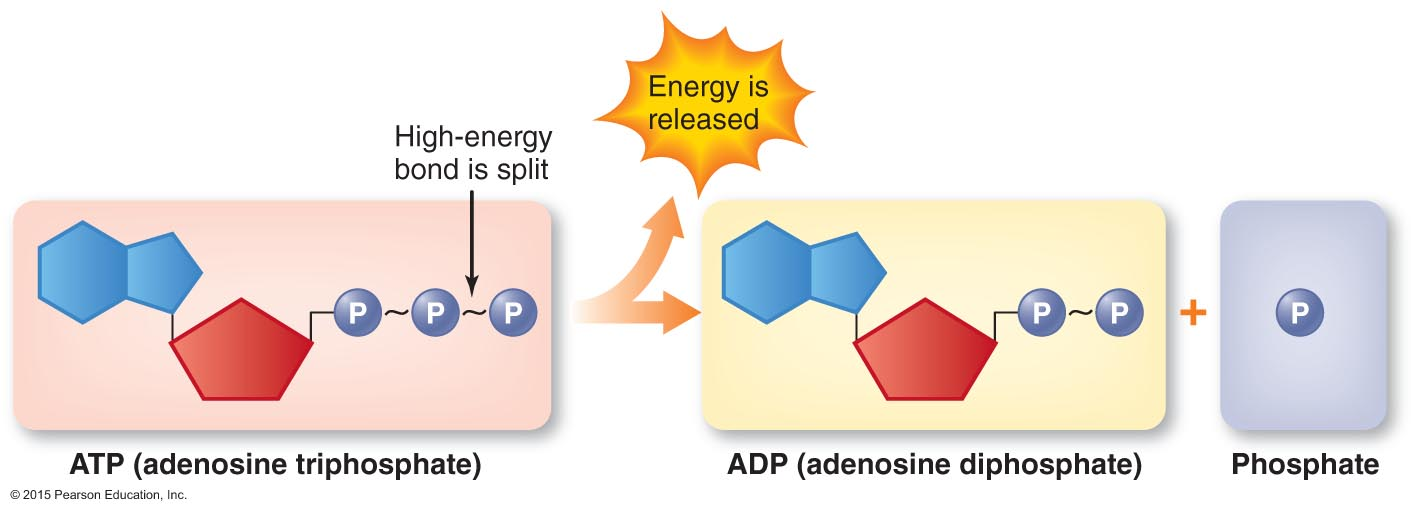
\includegraphics[width=\textwidth]{11_adenosine_triphosphate_atp}
	\caption{Adenosine Triphosphate (ATP)}
	\label{fig:atp}
\end{figure}

\begin{figure}[H]
	\centering
	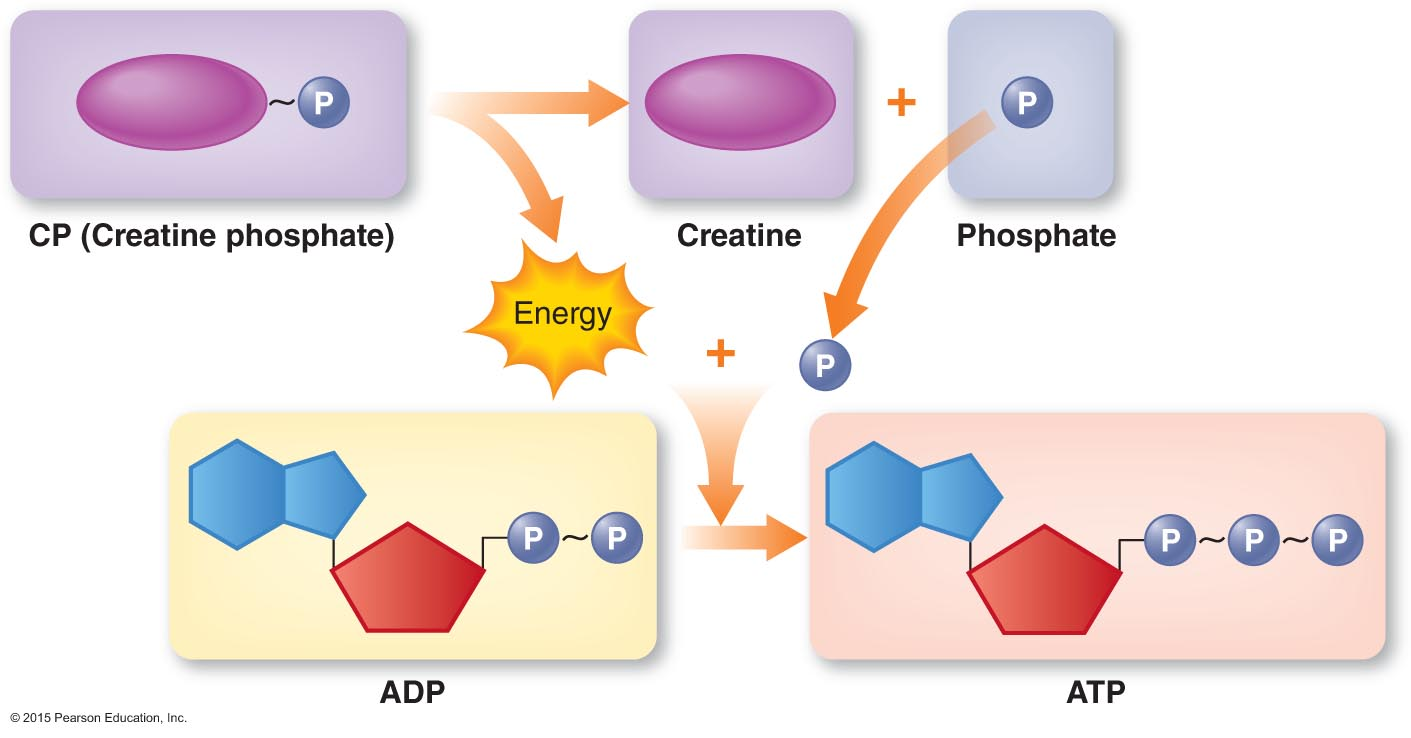
\includegraphics[width=\textwidth]{11_creatine_phosphate_cp}
	\caption{Creatine Phosphate (CP)}
	\label{fig:creatine-phosphate}
\end{figure}

\begin{figure}[H]
	\centering
	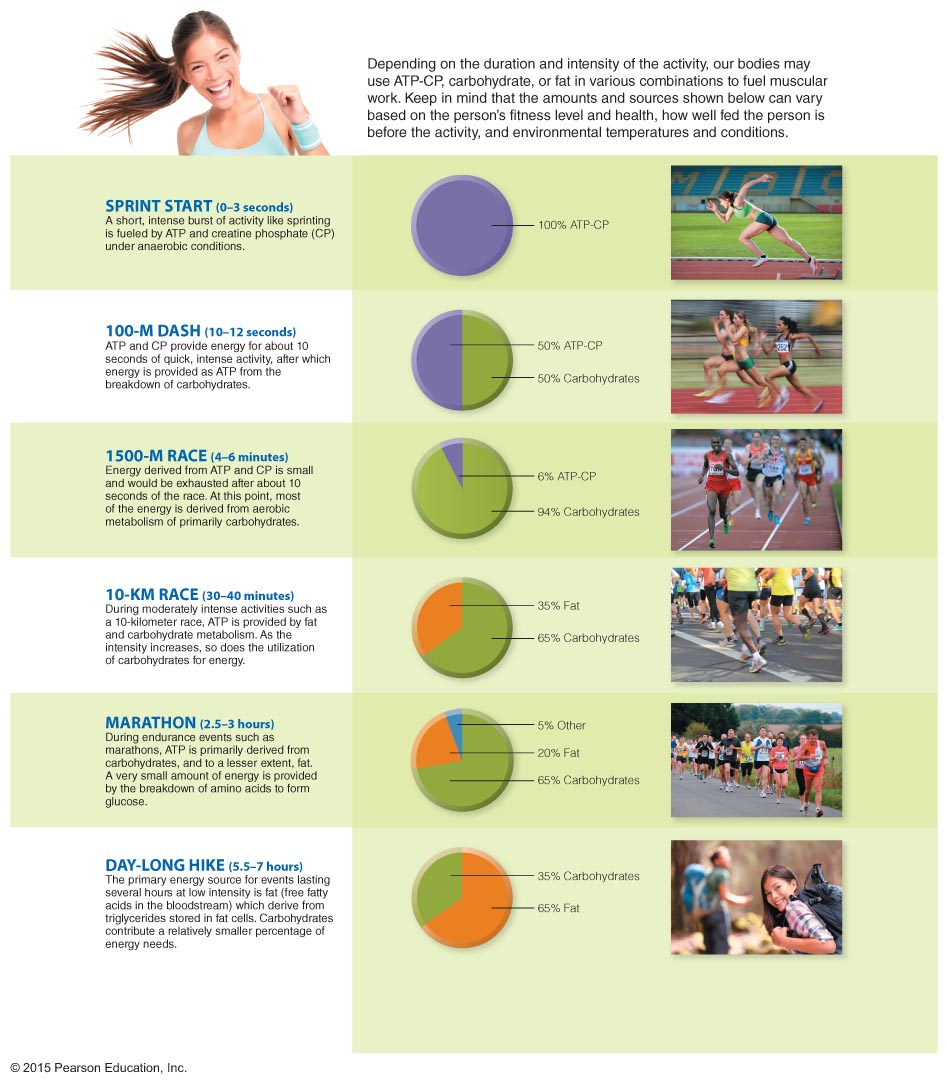
\includegraphics[width=\textwidth]{11_energy_balance}
	\caption{Energy Balance}
	\label{fig:energy-balance}
\end{figure}

\begin{itemize}
	\item Metabolism of glucose
	\begin{itemize}
		\item \emph{Anaerobic} (without oxygen) breakdown of glucose yields two ATP molecules
		\begin{itemize}
			\item Lactic acid is produced
		\end{itemize}
	\end{itemize}
	\begin{itemize}
		\item \emph{Aerobic} (with oxygen) breakdown of glucose yields 36--38 molecules of ATP
		\begin{itemize}
			\item $\mbox{CO}_{2}$ and $\mbox{H}_{2}$O are produced
		\end{itemize}
	\end{itemize}
\end{itemize}

\begin{figure}[H]
	\centering
	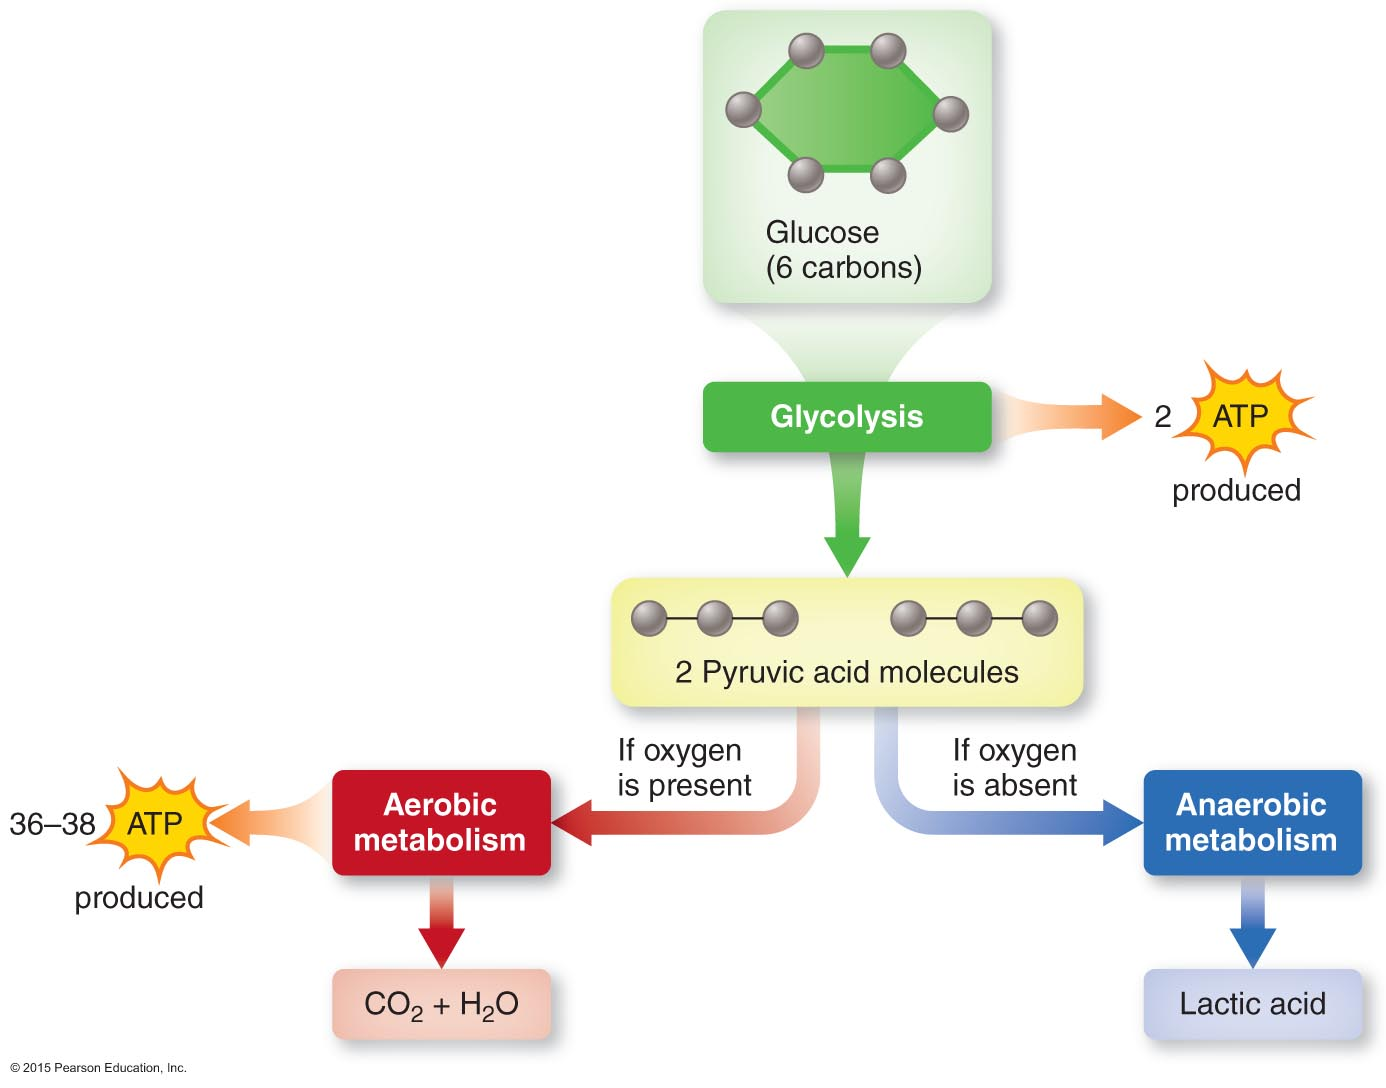
\includegraphics[width=\textwidth]{11_metabolism_of_glucose}
	\caption{Metabolism of Glucose}
	\label{fig:metabolism-of-glucose}
\end{figure}

\begin{itemize}
	\item Stored triglycerides (fats) can be metabolized to generate ATP
	\begin{itemize}
		\item For low-intensity exercise
		\item For exercise of long duration
		\item A very abundant energy source, even in lean people
		\item Provides more than two times the energy per gram as carbohydrate
	\end{itemize}
	\item Carbohydrates and fats can both be used as energy sources for the production of ATP
	\begin{itemize}
		\item Carbohydrates are mostly used for high-intensity activity
		\item Fats are used for low-intensity exercise
	\end{itemize}
	\item Proteins (amino acids) are not a major fuel source for exercise
	\begin{itemize}
		\item 1--6\% of energy needs during exercise
	\end{itemize}
\end{itemize}

\begin{figure}[H]
	\centering
	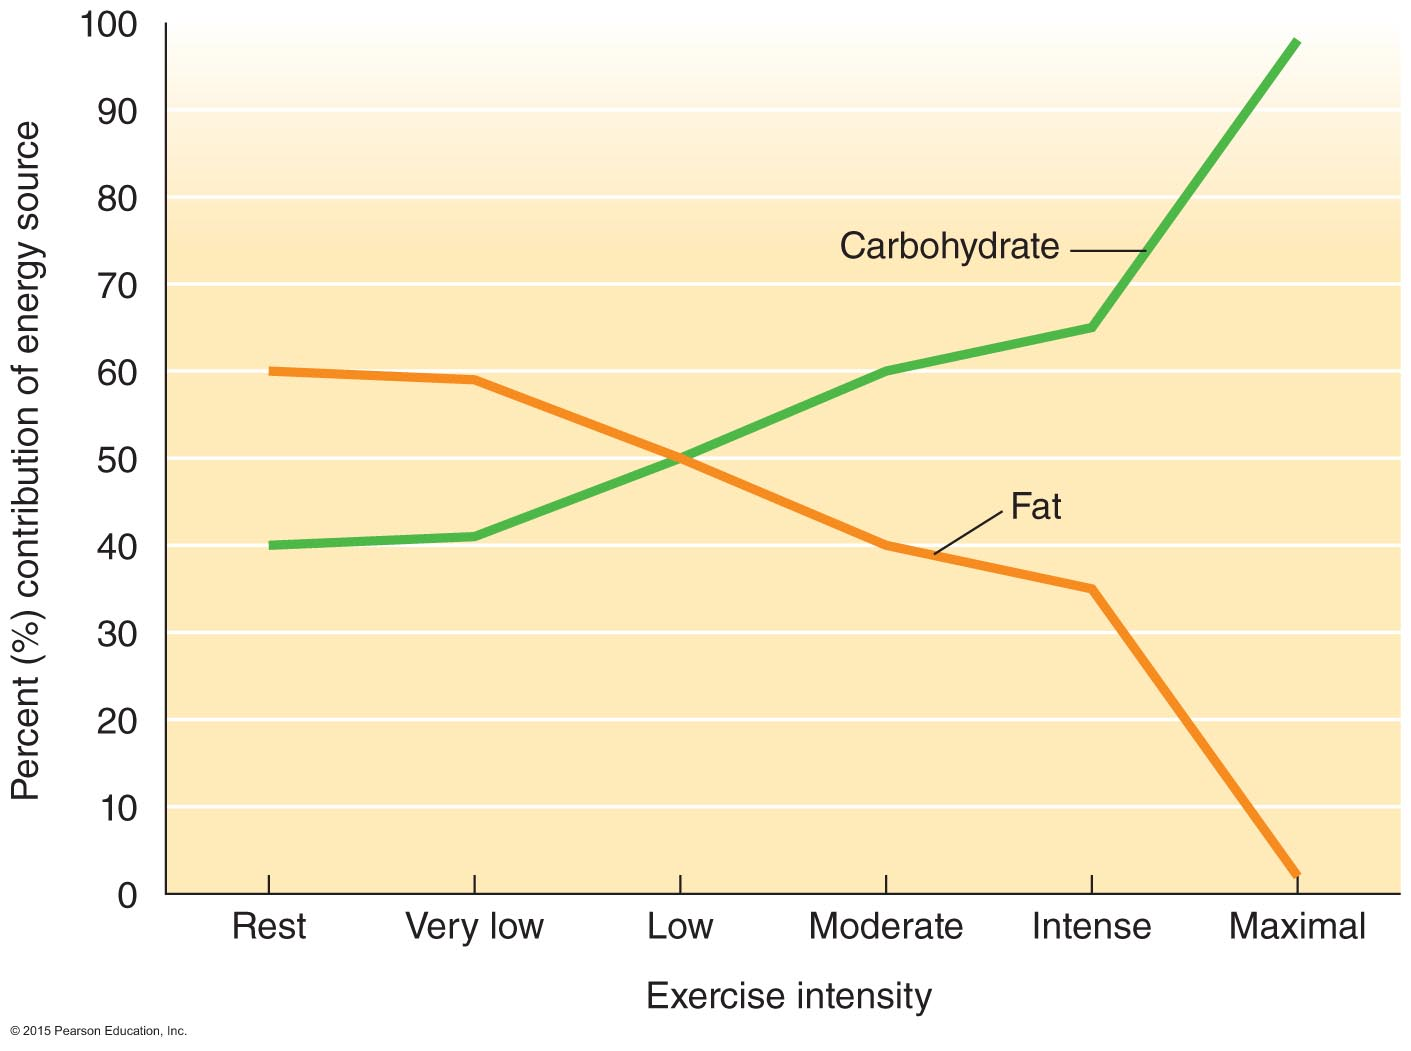
\includegraphics[width=\textwidth]{11_fat_and_carbohydrate_contributions}
	\caption{Fat and Carbohydrate Contributions}
	\label{fig:fat-and-carbohydrate-contributions}
\end{figure}

\begin{figure}[H]
	\centering
	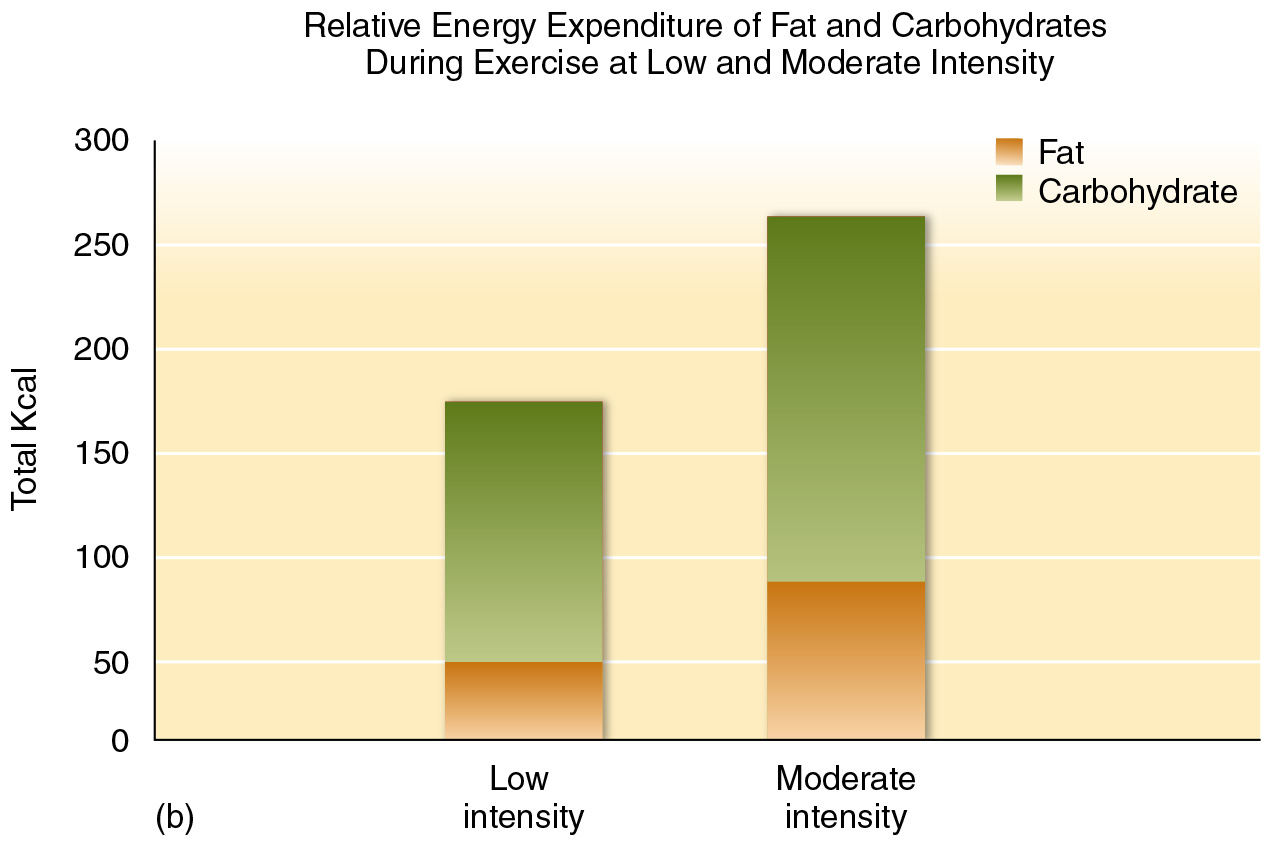
\includegraphics[width=\textwidth]{11_fat_and_carbohydrate_contributions_2}
	\caption{Fat and Carbohydrate Contributions (cont.)}
	\label{fig:fat-and-carbohydrate-contributions-2}
\end{figure}

\section{Energy Needs for Physical Activity}\label{sec:energy-needs-for-physical-activity}
\begin{itemize}
	\item Energy needs
	\begin{itemize}
		\item Energy needs may be higher for athletes
		\item Different energy needs for males and females
		\item Depend on body size
		\item Depend on the type, intensity, and duration of physical activity
	\end{itemize}
\end{itemize}

\nutrients{Nutrients for Vigorous Physical Activity}{tab:nutrients-for-vigorous-physical-activity}

\begin{figure}[H]
	\centering
	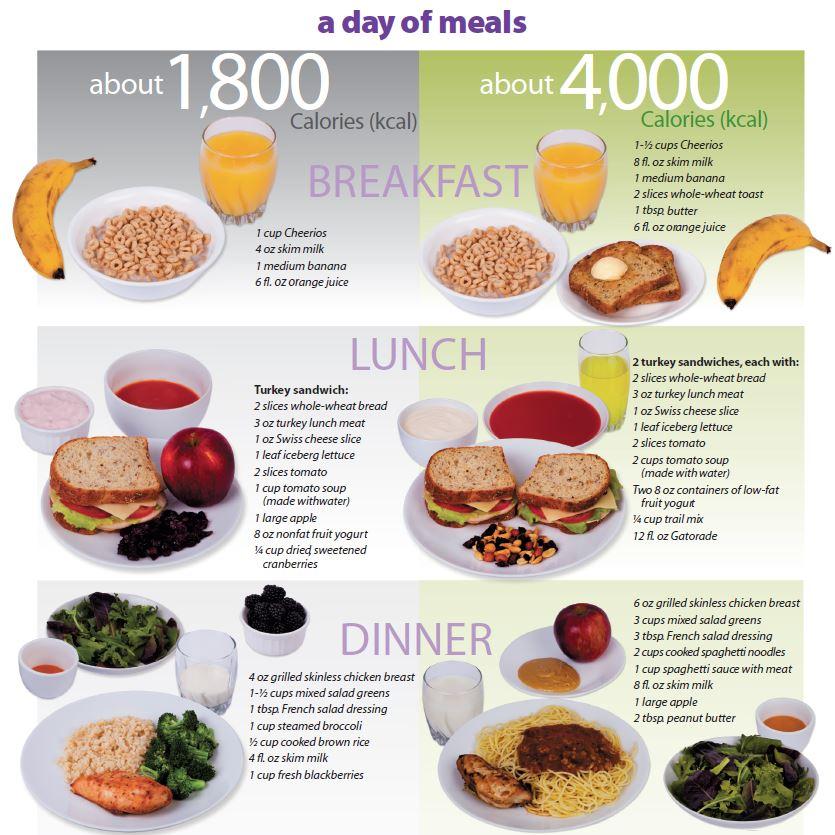
\includegraphics[width=\textwidth]{11_eating_for_athletes}
	\caption{Eating for Athletes}
	\label{fig:eating-for-athletes}
\end{figure}

\section{Carbohydrate Intake for Physical Activity}\label{sec:carbohydrate-intake-for-physical-activity}
\begin{itemize}
	\item Athletes should consume carbohydrate within the AMDR of 45--65\% of total energy intake
	\item Athletes should consume a daily carbohydrate intake of 6--10 grams per kg body weight to optimize glycogen stores
	\item Good sources are fiber-rich, less-processed foods such as whole grains, cereals, vegetables, and juices
\end{itemize}

\begin{figure}[H]
	\centering
	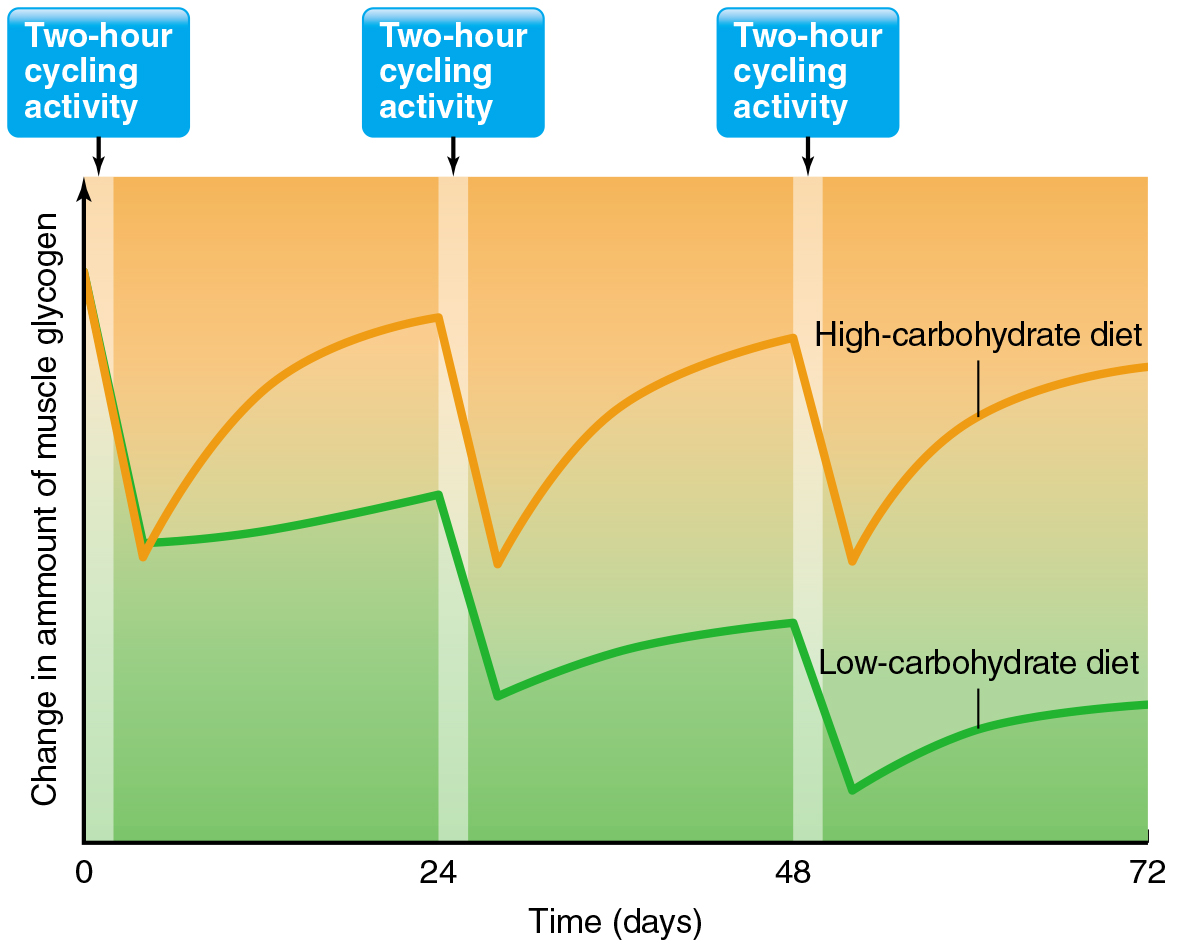
\includegraphics[width=\textwidth]{11_carbohydrates_and_muscle_glycogen_stores}
	\caption{Carbohydrates and Muscle Glycogen Stores}
	\label{fig:carbohydrates-and-muscle-glycogen-stores}
\end{figure}

\begin{table}[H]
	\centering
	\begin{threeparttable}
		\caption{Carbohydrate and Total energy in Various Foods}
		\label{tab:carbohydrate-and-total-energy-in-various-foods}
		\rowcolors{2}{rowmedgreen}{rowlightgreen}
		\begin{tabular}{p{0.275\textwidth} p{0.1\textwidth}p{0.2\textwidth}p{0.2\textwidth} p{0.2\textwidth}}
			\rowcolor{rowdarkgreen}\textbf{Food} & \textbf{Amount} & \textbf{Carbohydrate (g)} & \textbf{Energy from Carbohydrate (\%)} & \textbf{Total Energy (kcal)}\\
			Sweetened applesauce & 1 cup				& 50 & 97 & 207\\
			Large apple with & 1 each					& 50 & 82 & 248\\
			saltine crackers & 8 each					& & & \\
			Whole-wheat bread & 1-oz slice				& 50 & 71 & 282\\
			with jelly & 4 tsp.							& & & \\
			and skim milk & 12 fl. oz					& & & \\
			Spaghetti (cooked) & 1 cup					& 50 & 75 & 268\\
			with tomato sauce  & $\frac{1}{4}$ cup		& & & \\
			Brown rice (cooked) & 1 cup					& 100 & 88 & 450\\
			with mixed vegetables & $\frac{1}{2}$ cup	& & & \\
			and apple juice & 12 fl. oz					& & & \\
			Grape-Nuts cereal & $\frac{1}{2}$ cup		& 100 & 84 & 473\\
			with raisins & $\frac{3}{8}$ cup			& & &\\
			and skim milk & 8 fl. oz					& & &\\
			Clif Bar (chocolate chip) & 2.4 oz			& 43 & 75 & 230\\
			Meta-Rx (fudge brownie) & 100 g				& 41 & 41 & 400\\
			Power Bar (chocolate) & 1 bar				& 45 & 75 & 240\\
			PR Bar Ironman & 1 bar						& 22 & 44 & 200\\
			\rowcolor{rowdarkgreen} & & & & \\
		\end{tabular}
		\begin{tablenotes}
			\small
			\item Source: Data adapted from Manore, M. M., N. L. Meyer, and J. L. Thompson. 2009. Sport Nutrition for Health and Performance, 2nd ed. Champaign, IL: Human Kinetics.
		\end{tablenotes}
	\end{threeparttable}
\end{table}

\begin{itemize}
	\item \emph{Carbohydrate loading}, or glycogen loading, involves altering training and carbohydrate intake so that muscle glycogen storage is maximized
	\begin{itemize}
		\item May benefit athletes competing in marathons, distance swimming, cross-country skiing, and triathlons
		\item Does not always improve performance
		\item Can lead to adverse side effects
	\end{itemize}
\end{itemize}

\begin{table}[H]
	\centering
	\begin{threeparttable}
		\caption{Carbohydrate Loading Guidelines}
		\label{tab:carbohydrate-loading-guidelines}
		\rowcolors{2}{rowmedgreen}{rowlightgreen}
		\begin{tabular}{p{0.26\textwidth}p{0.32\textwidth}p{0.32\textwidth}}
			\rowcolor{rowdarkgreen}\textbf{Days Prior to Event} & \textbf{Exercise Duration (in minutes)} & \textbf{Carbohydrate Content of Diet (g per kg body weight)}\\
				6 & 90 (at 90\% max effort) & 5 (moderate)\\
				5 & 40 (at 70\% max effort) & 5 (moderate)\\
				4 & 40 (at 70\% max effort) & 5 (moderate)\\
				3 & 20 (light training) & 10--12 (high)\\
				2 & 20 (light training) & 10--12 (high)\\
				1 & Rest & 10--12 (high)\\
				Day of race & Competition & Pre-competition food and fluid\\
			\rowcolor{rowdarkgreen} & & \\
		\end{tabular}
		\begin{tablenotes}
			\small
			\item Sources: Current Trends in Performance Nutrition, by Marie Dunford. Copyright © 2005 by Human Kinetics, Champaign, IL. Reprinted with permission; and American College of Sports Medicine, Academy of Nutrition and Dietetics, and Dietitians of Canada. 2016. Nutrition and Athletic Performance. Joint Position Statement. Medicine and Science in Sports and Exercise 48(3):543-568.
		\end{tablenotes}
	\end{threeparttable}
\end{table}

\section{Fat Intake for Physical Activity}\label{sec:fat-intake-for-physical-activity}
\begin{itemize}
	\item Fat intake of 20--35\% of total energy intake is generally recommended for both athletes and non-athletes, with less than 10\% as saturated fat
	\item Fat provides energy, fat-soluble vitamins, and essential fatty acids
	\begin{itemize}
		\item Inadequate levels can prove detrimental to training and performance
	\end{itemize}
\end{itemize}

\section{Protein Intake for Physical Activity}\label{sec:protein-intake-for-physical-activity}
\begin{itemize}
	\item Protein intakes suggested for active people range from 1.2 to 2.0 grams per kg of body weight
	\item High-quality sources include lean meats, poultry, fish, eggs, low-fat dairy products, legumes, and soy products
\end{itemize}

\section{Fluid Intake for Physical Activity}\label{sec:fluid-intake-for-physical-activity}
\begin{itemize}
	\item Fluids
	\begin{itemize}
		\item Enable the body’s primary cooling mechanism, \emph{evaporative cooling}
		\item Are necessary to prevent dehydration and heat-related illnesses
	\end{itemize}
	\item Fluid intake is critical for physically active people
	\begin{itemize}
		\item Drink fluids before, during, and after exercise
		\item Consume enough to maintain body weight
		\item Training in hot environments requires careful attention to water intake
	\end{itemize}
\end{itemize}

\section{Fluid Intake and Physical Activity}\label{sec:fluid-intake-and-physical-activity}
\begin{itemize}
	\item Heat production during exercise can increase 15 to 20 times compared to inactivity
	\item The body cools itself through evaporative cooling, but heat illness can occur with dehydration
	\begin{itemize}
		\item Heat syncope
		\item Heat cramps
		\item Heat exhaustion
	\end{itemize}
\end{itemize}

\begin{figure}[H]
	\centering
	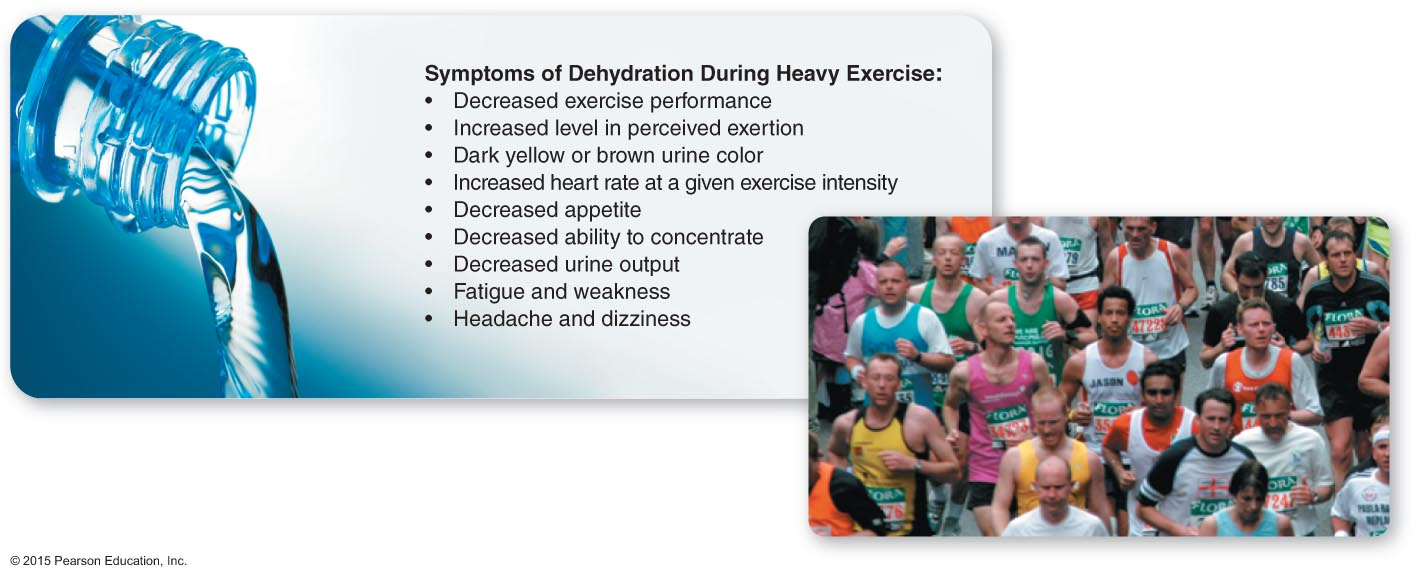
\includegraphics[width=\textwidth]{11_dehydration_symptoms}
	\caption{Dehydration Symptoms}
	\label{fig:dehydration-symptoms}
\end{figure}

\begin{table}[H]
	\centering
	\begin{threeparttable}
		\caption{Guidelines for Fluid Replacement}
		\label{tab:guidelines-for-fluid-replacement}
		\rowcolors{2}{rowmedgreen}{rowlightgreen}
		\begin{tabular}{p{0.225\textwidth}p{0.225\textwidth}p{0.5\textwidth}}
			\rowcolor{rowdarkgreen}\textbf{Activity Level} & \textbf{Environment} & \textbf{Fluid Requirements (liters per day)}\\
			Sedentary & Cool & 2--3\\
			Active & Cool & 3--6\\
			Sedentary & Warm & 3--5\\
			Active & Warm & 5--10\\
			\multicolumn{3}{p{\textwidth}}{\textbf{Before Exercise or Competition}
				\begin{itemize}
					\item Drink adequate fluids during the 24 hours before event; should be able to maintain body weight.
					\item Slowly drink about 0.17 to 0.34 fl.\ oz per kg body weight of water or a sports drink in the 2 to 4 hours prior to exercise or event to achieve urine that is pale yellow in color while allowing sufficient time for excretion of excess fluid prior to exercise.
					\item Consuming beverages with sodium and/or small amounts of salted snacks at a meal will help stimulate thirst and retain fluids consumed.
				\end{itemize}}~\\
			\multicolumn{3}{p{\textwidth}}{\textbf{During Exercise or Competition}
				\begin{itemize}
					\item Amount and rate of fluid replacement depend on individual sweating rate, exercise duration, weather conditions, and opportunities to drink.
					\item Drink sufficient fluids during exercise to replace sweat losses such that total fluid loss is less than 2\% of body weight.
				\end{itemize}}~\\
			\multicolumn{3}{p{\textwidth}}{\textbf{Following Exercise or Competition}
				\begin{itemize}
					\item Consume about 3 cups of fluid for each pound of body weight lost.
					\item Fluids after exercise should contain water to restore hydration status and sodium to support rehydration.
					\item Consume enough fluid to permit regular urination and to ensure the urine color is very light or light yellow in color; drinking about 125--150\% of fluid loss is usually sufficient to ensure complete rehydration.
				\end{itemize}}~\\
			\multicolumn{3}{p{\textwidth}}{\textbf{In General}
				\begin{itemize}
					\item Products that contain fructose should be limited, as these may cause gastrointestinal distress.
					\item Alcohol should be avoided, as it increases urine output and reduces fluid retention.
				\end{itemize}}~\\
			\rowcolor{rowdarkgreen} & &
		\end{tabular}
		\begin{tablenotes}
			\small
			\item Source: American College of Sports Medicine, Academy of Nutrition and Dietetics, and Dietitians of Canada. 2016. Nutrition and Athletic Performance. Joint Position Statement. Medicine and Science in Sports and Exercise 48(3):543-568.
		\end{tablenotes}
	\end{threeparttable}
\end{table}

\section{Micronutrient Intake for Physical Activity}\label{sec:micronutrient-intake-for-physical-activity}
\begin{itemize}
	\item The requirements for some vitamins and minerals may be elevated in athletes
	\begin{itemize}
		\item B-vitamins
		\item Calcium
		\item Iron
	\end{itemize}
	\item Adequate intake of these nutrients can be met with a healthy, balanced diet and should not require supplementation
\end{itemize}

\section{Ergogenic Aids}\label{sec:ergogenic-aids}
\begin{itemize}
	\item \definition{Ergogenic aids:}{substances used to improve exercise and athletic performance}
	\begin{itemize}
		\item Many of these products are not effective
		\item Some of these products are dangerous
		\item Reliable research and accurate information on these products are hard to find
	\end{itemize}
	\item Ergogenic aids used to build muscles and increase strength include
	\begin{itemize}
		\item Anabolic steroids
		\begin{itemize}
			\item Effective but illegal; numerous serious side effects
		\end{itemize}
	\end{itemize}
	\begin{itemize}
		\item Andro (androstenedione) and DHEA (dehydroepiandrosterone)
		\begin{itemize}
			\item Precursors of testosterone
			\item Not been shown to be effective
		\end{itemize}
	\end{itemize}
	\begin{itemize}
		\item GHB (gamma-hydroxybutyric acid)
		\begin{itemize}
			\item Severe side effects and some reported deaths
		\end{itemize}
	\end{itemize}
	\item Creatine
	\begin{itemize}
		\item It may improve performance in sprint activities
		\item It may be beneficial to increase strength gained during resistance exercise
		\item Relatively minor side effects
		\item Effects of long-term use are unknown
	\end{itemize}
	\item Protein and amino acid supplements
	\begin{itemize}
		\item Not been shown to be effective
	\end{itemize}
	\item Ergogenic aids used to increase energy levels and optimize fuel use include
	\begin{itemize}
		\item Caffeine
		\begin{itemize}
			\item Increases fat use for energy during exercise
			\item In energy drinks, associated with serious side effects in children, adolescents, and young adults
		\end{itemize}
		\item Ephedrine
		\begin{itemize}
			\item Stimulant banned in the United States
			\item Serious side effects and some reported deaths
			\item Also known as ephedra and ma huang
		\end{itemize}
	\end{itemize}
	\item Ergogenic aids found to be ineffective include
	\begin{itemize}
		\item Carnitine
		\begin{itemize}
			\item Claimed to increase transport of fatty acids into the mitochondria so they can be used for energy
		\end{itemize}
	\end{itemize}
	\begin{itemize}
		\item Chromium
		\begin{itemize}
			\item Claimed to enhance insulin’s action
		\end{itemize}
	\end{itemize}
	\begin{itemize}
		\item Ribose
		\begin{itemize}
			\item Claimed to increase work output and speed up recovery time
		\end{itemize}
	\end{itemize}
	\item One more ergogenic aid that \emph{may} have beneficial effects:
	\begin{itemize}
		\item Beta-alanine
		\begin{itemize}
			\item Increases the production of carnosine
			\item Supplementation may enhance a person’s ability to perform short-term, high-intensity activity and may delay muscle fatigue
			\item Several weeks of supplementation are needed to affect performance
		\end{itemize}
	\end{itemize}
\end{itemize}

\section{In Depth: Disorders Related to Body Image, Eating, and Exercise}\label{sec:in-depth:-disorders-related-to-body-image-eating-and-exercise}
\begin{itemize}
	\item Disordered eating
	\begin{itemize}
		\item A variety of atypical eating behaviors that people use to achieve a lower body weight
		\begin{itemize}
			\item Ex: going on a diet, refusing to eat fat
		\end{itemize}
		\item Eating disorder
		\begin{itemize}
			\item A psychiatric condition that involves extreme body dissatisfaction and long-term eating patterns that negatively affect body functioning
		\end{itemize}
	\end{itemize}
\end{itemize}

\subsection{Body Image}\label{subsec:body-image}
\begin{itemize}
	\item Body image
	\begin{itemize}
		\item A person’s perception, feelings about, and critique of his or her body’s appearance and functioning
	\end{itemize}
	\item Body image can affect eating and exercise behaviors
\end{itemize}

\begin{figure}[H]
	\centering
	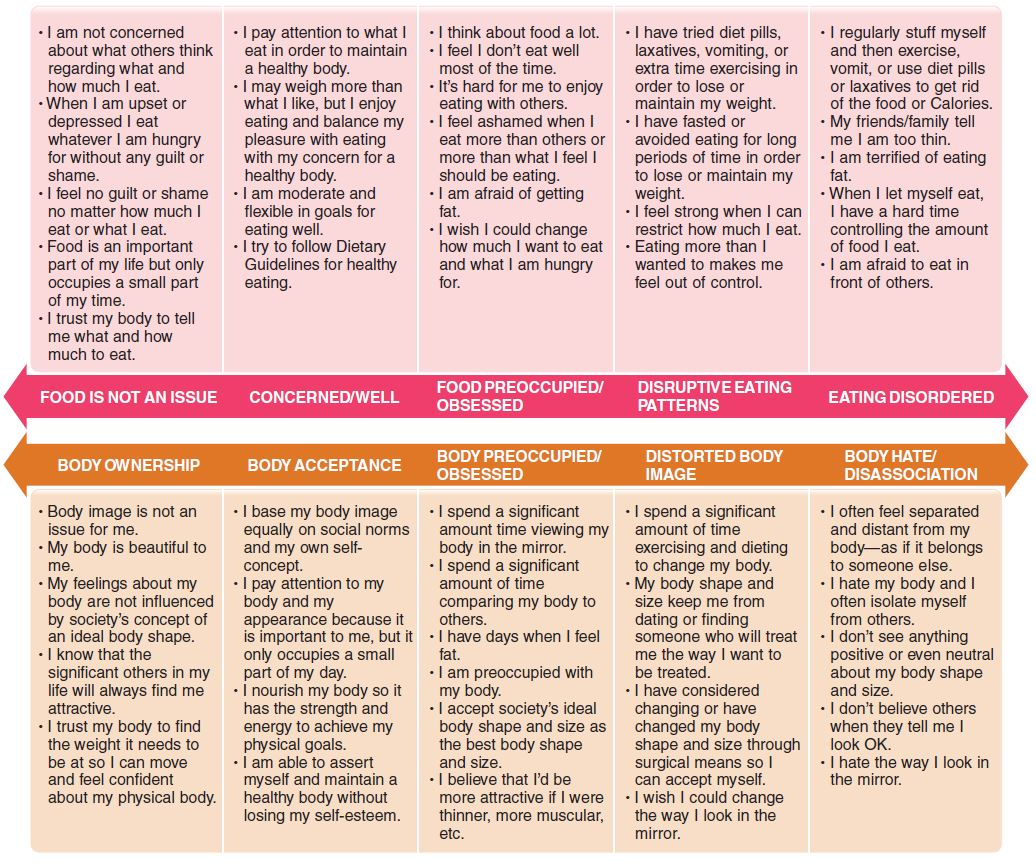
\includegraphics[width=\textwidth]{11_body_image}
	\caption{Body Image}
	\label{fig:body-image}
\end{figure}

\subsection{Body Dysmorphic Disorder}\label{subsec:body-dysmorphic-disorder}
\begin{itemize}
	\item Body dysmorphic disorder (BDD) is a clinically diagnosed psychiatric disorder characterized by a disabling preoccupation with perceived defects in appearance
	\begin{itemize}
		\item May affect up to 2.4\% of the population
		\item Equally common in males and females
	\end{itemize}
	\item Muscle dysmorphia
	\begin{itemize}
		\item Pathological pursuit of increased muscularity that causes individuals to engage in highly disordered eating behaviors
	\end{itemize}
\end{itemize}

\subsection{Contributing Factors}\label{subsec:contributing-factors}
\begin{itemize}
	\item Several factors may influence disorders related to body image, eating, and exercise
	\begin{itemize}
		\item Genetics
		\item Family environment
		\item Anxiety, compulsivity, abnormal eating behaviors
		\item Media
		\item Social/cultural values
		\item Other psychological disorders
	\end{itemize}
\end{itemize}

\subsection{Anorexia Nervosa}\label{subsec:anorexia-nervosa}
\begin{itemize}
	\item A serious, potentially life threatening eating disorder that is characterized by self-starvation
	\item Self-starvation can lead to deficiencies in essential nutrients and energy required for the human body to function normally
	\item Signs and symptoms
	\begin{itemize}
		\item Restrictive eating patterns
		\item Eliminating food groups
		\item Intense fear of weight gain
		\item Amenorrhea (loss of menstrual cycle for 3 months or more)
		\item Distorted body image
	\end{itemize}
	\item Health risks:
	\begin{itemize}
		\item Deficiency in total Calories and micronutrients
		\item Body will be forced to use fat stores and lean tissue for energy
		\item Reduction of non-vital bodily functions
		\item Electrolyte imbalances
		\begin{itemize}
			\item Can lead to heart failure or death
		\end{itemize}
	\end{itemize}
\end{itemize}

\begin{figure}[H]
	\centering
	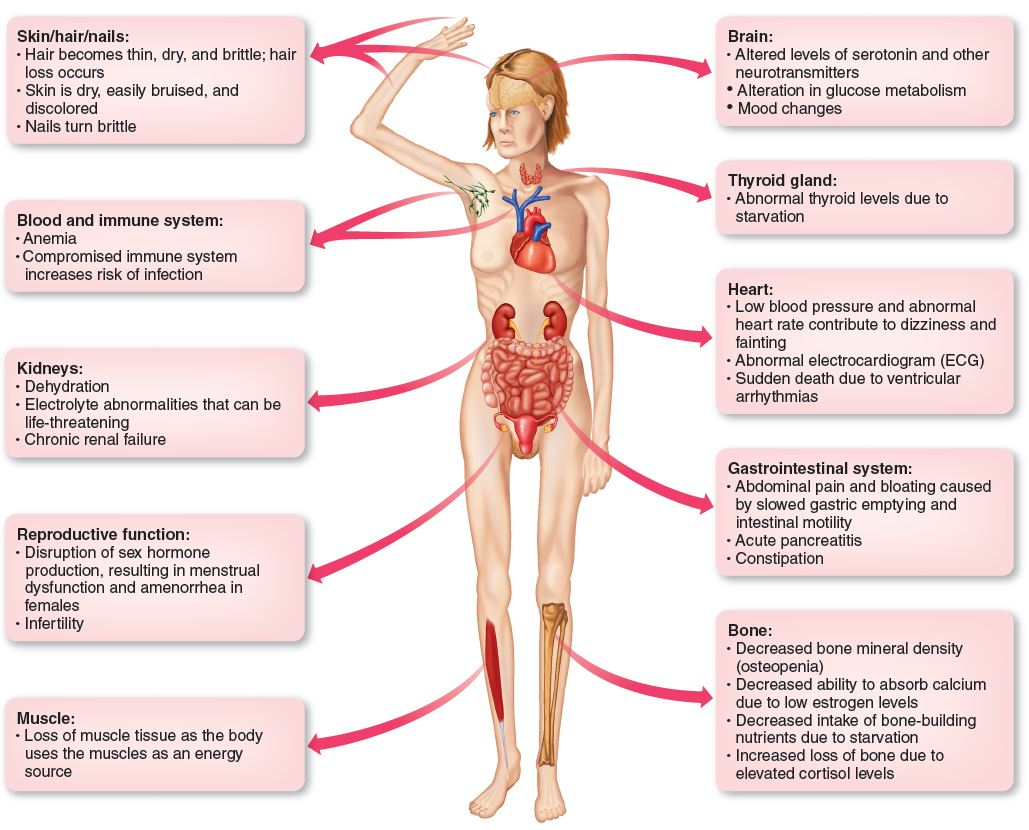
\includegraphics[width=\textwidth]{11_anorexia_nervosa}
	\caption{Anorexia Nervosa}
	\label{fig:anorexia-nervosa}
\end{figure}

\subsection{Bulimia Nervosa}\label{subsec:bulimia-nervosa}
\begin{itemize}
	\item Characterized by repeated episodes of binge eating and purging
	\begin{description}
		\item[Binge eating:] a consumption of a quantity of food that is large in size for the person and the amount of time in which the food is eaten
		\item[Purging:] compensatory behavior used to prevent weight gain. Methods include vomiting, laxative or diuretic abuse, enemas, fasting, and excessive exercise
	\end{description}
	\item Signs and symptoms
	\begin{itemize}
		\item Recurrent episodes of binge eating
		\item Recurrent inappropriate compensatory behavior in order to prevent weight gain
		\item Chronically inflamed and sore throat
		\item Swollen glands in the neck and jaw
		\item Worn tooth enamel
	\end{itemize}
	\item Health risks
	\begin{itemize}
		\item 3--5\% of adult female population
		\item 2\% of adult male population
		\item Increased risk of being overweight/obese due to increase in caloric consumption
		\item Increased blood lipids
		\item Low self-esteem
		\item Depression
	\end{itemize}
\end{itemize}

\subsection{Night-Eating Syndrome}\label{subsec:night-eating-syndrome}
\begin{itemize}
	\item A disorder characterized by intake of the majority of the days energy between 8 pm and 6 am
	\item Individuals with this disorder also experience mood and sleep disorders
\end{itemize}

\subsection{Female Athlete Triad}\label{subsec:female-athlete-triad}
\begin{itemize}
	\item Syndrome that consists of three clinical conditions in some physically active females
	\begin{itemize}
		\item Low energy availability
		\item Amenorrhea
		\item Low bone density
	\end{itemize}
	\item Typically seen in female athletes who participate in activities that emphasize leanness
\end{itemize}

%</Chapter11>

\end{document}
